\chapter[Utilização do eMAG no contexto do Projeto]{Utilização do eMAG no contexto do Projeto}
\label{chap:emag}

	O Modelo de Acessibilidade em Governo Eletrônico (eMAG) consiste em um conjunto de recomendações a ser considerado para que o processo de acessibilidade dos sítios e portais do governo brasileiro seja conduzido de forma padronizada e de fácil implementação.
	
	O eMAG foi conquistando tanto espaço, que em 2007, a Portaria nº 3, de 7 de maio, institucionalizou o eMAG no âmbito do Sistema de Administração dos Recursos de Tecnologia da Informação (SISP). Dessa maneira, a observância de suas recomendações passou a ser obrigatória nos sítios e portais do governo brasileiro.
	
	É importante ressaltar que a versão mais recente do modelo contou com contribuições de especialistas e as novas pesquisas na área de acessibilidade à Web, bem como as Recomendações de Acessibilidade para Conteúdo Web.

	O eMAG possui uma Legislação relativa a acessibilidade, dentre as leis e decretos, percebe-se:

	\begin{itemize}
		\item{Decreto Nº 7.724, de 16 de maio de 2012 – Regulamenta a Lei Nº 12.527, que dispõe sobre o acesso a informações;}
		\item{Decreto Nº 6.949, de 25 de agosto de 2009 – Promulga a Convenção Internacional sobre os Direitos das Pessoas com Deficiência e seu Protocolo Facultativo;}
		\item{Decreto Legislativo Nº 186, de 9 de julho de 2008 – Aprova o texto da Convenção sobre os Direitos das Pessoas com Deficiência e de seu Protocolo Facultativo, assinados em Nova Iorque, em 30 de março de 2007.}
	\end{itemize}

	É importante considerar que não são apenas esses decretos e leis, mas existem uma série de outros fatores correlatos, confirmando a importância de prestação de assistência às pessoas com deficiência.

	Contudo, é importante considerar que as recomendações do eMAG não auxiliam somente pessoas com deficiência, mas promove facilitações a qualquer grupo de usuários.

	\section[Aplicações]{Aplicações}
	\label{sec:emag_aplicacoes}

	Para o projeto foi necessário adotar as diretrizes de governo eletrônico para garantir os aspectos atreladas a usabilidade no tocante a versão \emph{website} da aplicação.	

	\newpage
	\begin{landscape}
	A seguir são apresentados as imagens do protótipo do \emph{website}.
	
	\begin{figure}[h]
		\centering
		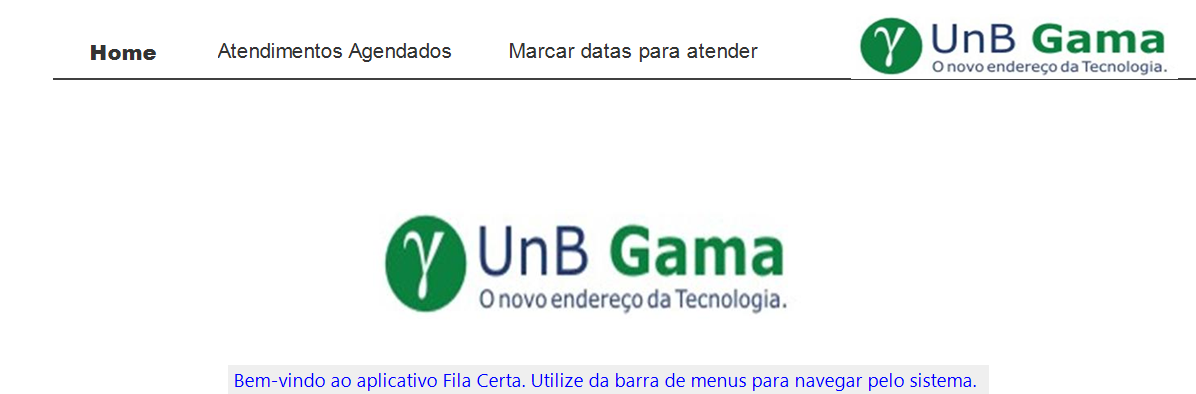
\includegraphics[scale=0.6]{emag1}
		\caption[Página Home do Protótipo Web]{Página Home do Protótipo \emph{Web}.}
		\label{fig:emag1}
	\end{figure}

	\begin{figure}[h]
		\centering
		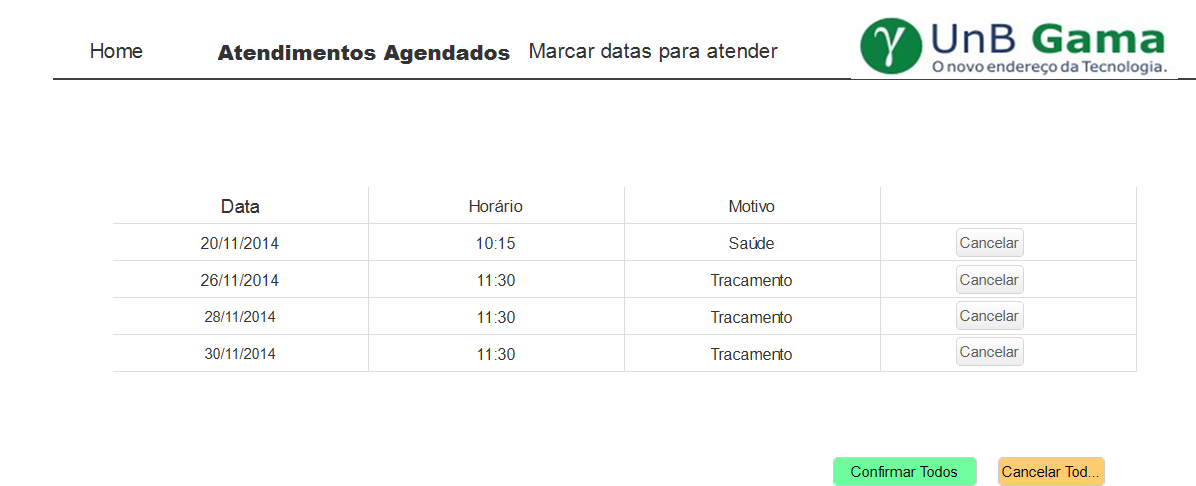
\includegraphics[scale=0.6]{emag2}
		\caption[Página de Consultas Agendadas do Protótipo Web]{Página de Consultas Agendadas do Protótipo \emph{Web}.}
		\label{fig:emag2}
	\end{figure}

	\begin{figure}[h]
		\centering
		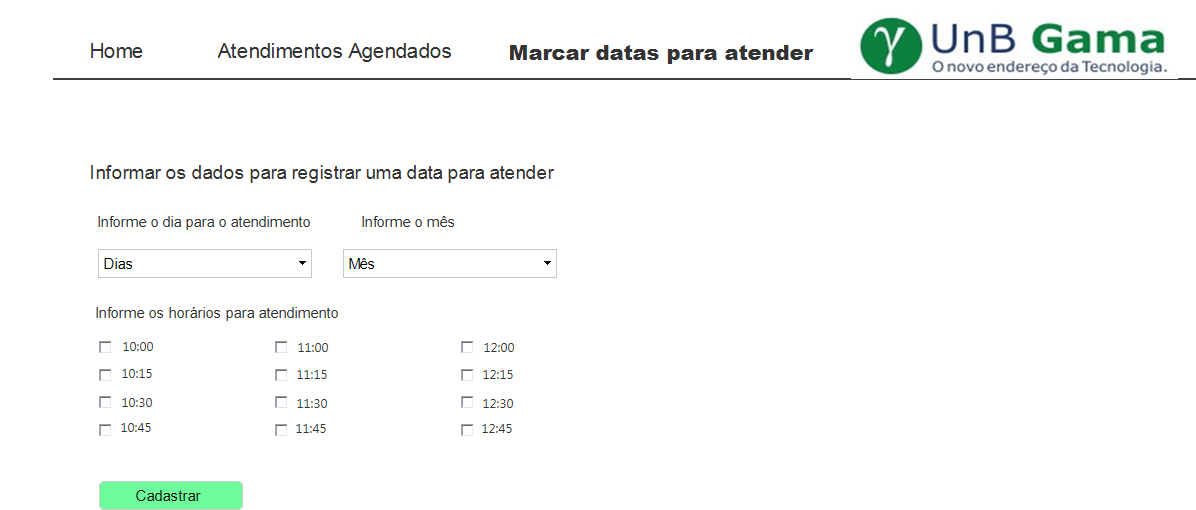
\includegraphics[scale=0.6]{emag3}
		\caption[Página de Cadastrar novo Atendimento do Protótipo Web]{Página de Cadastrar novo Atendimento do Protótipo \emph{Web}.}
		\label{fig:emag3}
	\end{figure}

	\begin{figure}[h]
		\centering
		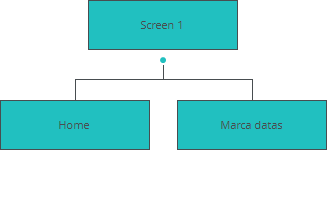
\includegraphics[scale=0.8]{emag4}
		\caption[Mapa das Páginas do Protótipo Web]{Mapa das Páginas do Protótipo \emph{Web}.}
		\label{fig:emag4}
	\end{figure}
	\end{landscape}

	\newpage
	\begin{landscape}
	
	Mesmo com a instalação do plugin \emph{eScanner} para avaliação com base nas diretrizes do eMAG para \emph{website}, não foi possível analisar o protótipo, pois a ferramenta não conseguiu reconhecer os códigos fontes dele, como pode ser observado na imagem a sguir.

	\begin{figure}[h]
		\centering
		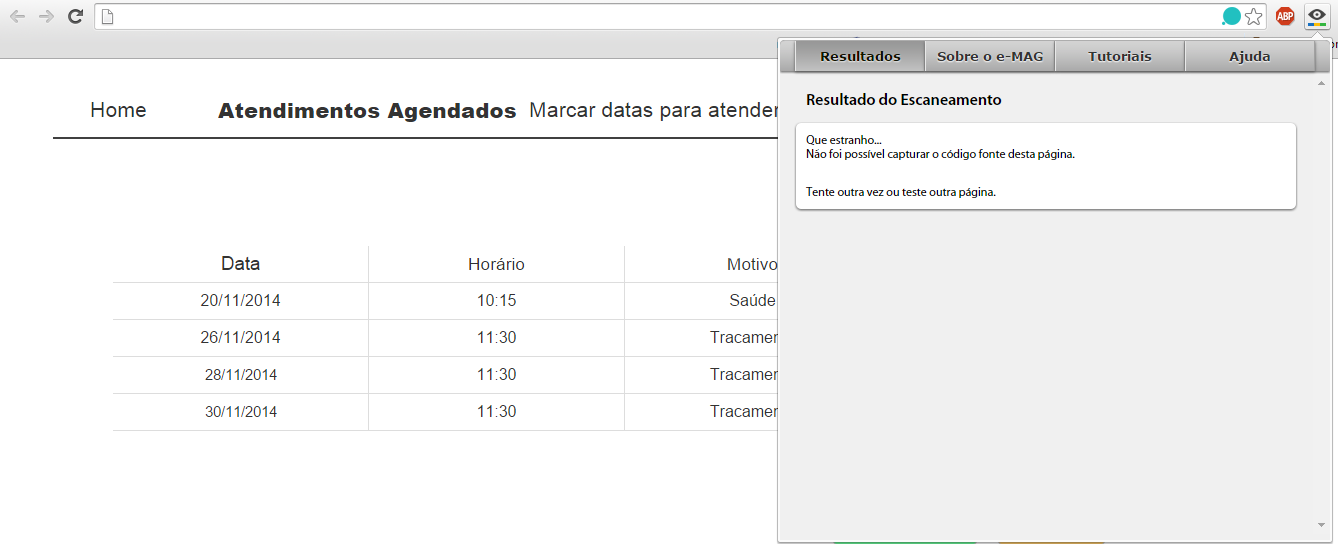
\includegraphics[scale=0.6]{emag5}
		\caption[Reconhecimento de Código - eScanner]{[Reconhecimento de Código - \emph{eScanner}.}
		\label{fig:emag5}
	\end{figure}
	\end{landscape}

	